\documentclass[a4paper, 12pt]{article}
\usepackage{graphicx}
\usepackage{listings}

\setlength\parindent{24pt}

\lstset{basicstyle=\footnotesize\ttfamily,breaklines=true, frame=single}

\begin{document}

\begin{figure}
    \centering
    
\includegraphics[width=1\textwidth]{Logo}
\end{figure}

\title{Assignment Report}
\author{Manwel Bugeja}
\date{\today}
\maketitle

\tableofcontents
\newpage

\section{Introduction}
\subsection{Note on the code}
This assignment is implemented in c++. Readability was prioritized over efficiency since the code needs to be
easily understood by others. 

\section{Part 1}
\subsection{How the problem was tackled}
\subsubsection{Structures}
First off, the needed structures where created: 'literal\_e' in an enumerated type containing the possible variables along with their negation.
An 'inv' literal was also created whose use is for error catching purposes.

Then a clause was defined as a vector of literals. Similarly, a formula was defined as a vector of clauses.

Apart from those, 'expression\_t' was also defined as an array of alphabet. Alphabet being an enumeration
containing the possible alphabet characters received as input.

These structures are defined in 'formula.h'.

\subsubsection{Parsing}
In the parsing, the string is first converted to an 'expression\_t'. Then it is translated to a formula. Since all variables are 
only a character long, the commas can be ignored completly when the expression is inputted. For example "(wx), (!w)" will still be parsed successfully. 
This will not reslut in an error as the input can still be successfully parse. 
Still, inserting "(," will still cause the program to exit since after an open parethesis, 
the parser expects a literal (variable or negation followed by a variable).

\subsection{The DPLL algorithm}
The DPLL algorithm was implemented according to the pseudo code listed in the course notes. In the 'choose\_literal()' part of the algorithm,
the first literal from the left is chosen.

\subsection{Testing}
For the testing of the algorithm, some expressions where tried, with the output compared. Included in this document are examples from the notes.

\begin{lstlisting}[caption=1-literal rule test]
$ ./part_1_binary
Hello, World!
Enter expression
(w), (!w, x)
RECIVED INPUT: (w), (!w, x)
Checking if input is alphabetically correct
Checking if syntax is valid
Printing formula
w
!w x
Running algorithm
Starting DPLL
w
!w x
Removing trivially sat
w
!w x
Applying one lit rule
Applying pure lit rule
SAT
\end{lstlisting}

\begin{lstlisting}[caption=pure literal rule test]
$ ./part_1_binary
Hello, World!
Enter expression
(w, x), (w, y), (!x, !y)
RECIVED INPUT: (w, x), (w, y), (!x, !y)
Checking if input is alphabetically correct
Checking if syntax is valid
Printing formula
w x
w y
!x !y
Running algorithm
Starting DPLL
w x
w y
!x !y
Removing trivially sat
w x
w y
!x !y
Applying one lit rule
w x
w y
!x !y
Applying pure lit rule
!x !y
Starting DPLL
!x !y
!x
Removing trivially sat
!x !y
!x
Applying one lit rule
!x !y
Applying pure lit rule
SAT
\end{lstlisting}

\begin{lstlisting}[caption=DPLL recursion test]
$ ./part_1_binary
Hello, World!
Enter expression
(x, y, z), (x, !y), (y, !z), (z, !x), (!x, !y, !z)
RECIVED INPUT: (x, y, z), (x, !y), (y, !z), (z, !x), (!x, !y, !z)
Checking if input is alphabetically correct
Checking if syntax is valid
Printing formula
x y z
x !y
y !z
z !x
!x !y !z
Running algorithm
Starting DPLL
x y z
x !y
y !z
z !x
!x !y !z
Removing trivially sat
x y z
x !y
y !z
z !x
!x !y !z
Applying one lit rule
x y z
x !y
y !z
z !x
!x !y !z
Applying pure lit rule
x y z
x !y
y !z
z !x
!x !y !z
Starting DPLL
x y z
x !y
y !z
z !x
!x !y !z
x
Removing trivially sat
x y z
x !y
y !z
z !x
!x !y !z
x
Applying one lit rule
x y z

Applying pure lit rule

Starting DPLL
x y z
x !y
y !z
z !x
!x !y !z
!x
Removing trivially sat
x y z
x !y
y !z
z !x
!x !y !z
!x
Applying one lit rule

z !x
!x !y
Applying pure lit rule

UNSAT
\end{lstlisting}

\section{Part 2}
\subsection{How the problem was tackled}
First off, the input is checked for any invalid characters, printing an error if any are found.
In the huffman algorithm, the input is iterated and the values are stored in a map. The map contains the character
and the corresponding weight.

Following that, the map is translated to a vector of nodes (which are all leaves at this point in time).
Then, a while loop is used to attach the least two nodes together. An '\_' is used as a character for non leaf nodes.
The nodes which were merged are removed from the vector. The new node is then added to the vector. The while loop 
goes on until the vector consists of one element i.e. the root node.

\subsection{Testing}
For testing, some outputs where tested manually by hand. Online generators where also used to compare the output. Included are
a sample output of the program and the tree obtained by an online generator. The output match but the values are flipped.


\begin{figure}
    \centering
    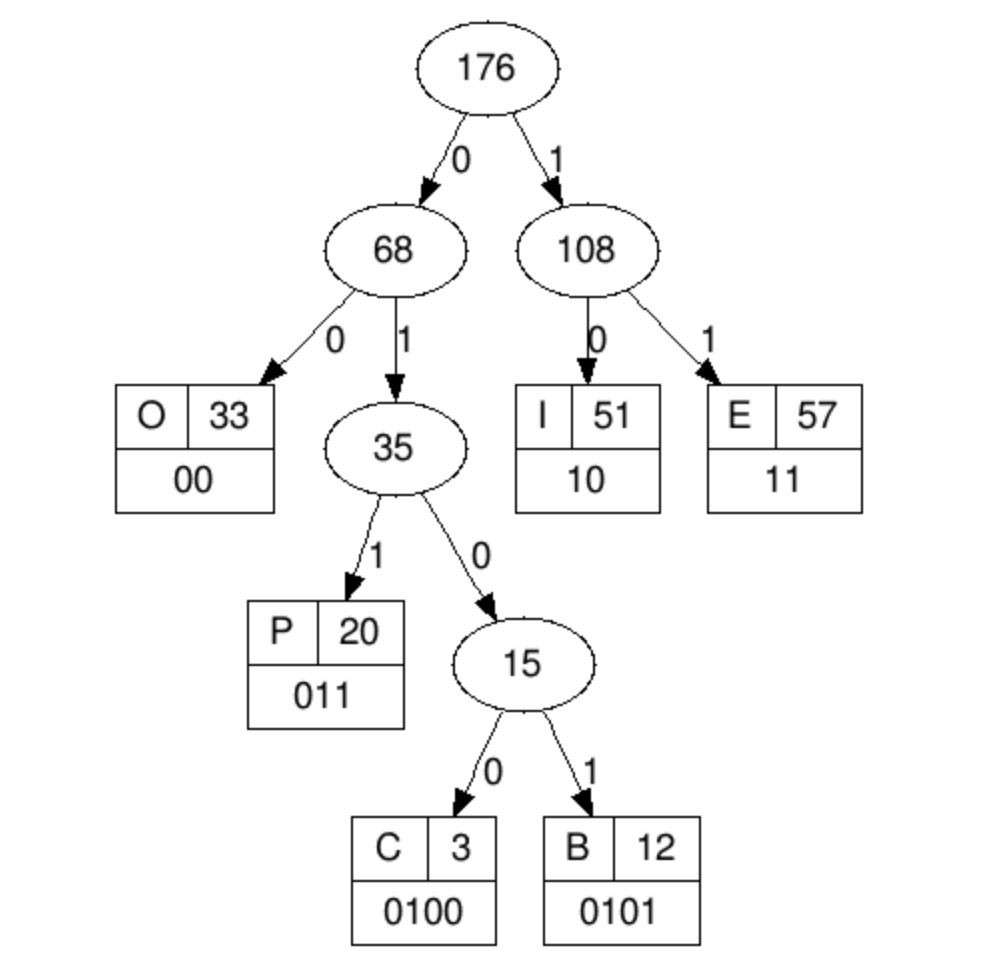
\includegraphics[width=1\textwidth]{huffman_1}
    \caption{Website used: http://huffman.ooz.ie/}
\end{figure}

\begin{lstlisting}[caption=Program output]
$ ./part_2_binary input
Hello, World!
Building tree:
Compressing: bbbbbbbbbbbbccceeeeeeeeeeeeeeeeeeeeeee
eeeeeeeeeeeeeeeeeeeeeeeeeeeeeeeeeeiiiiiiiiiiiiiiiii
iiiiiiiiiiiiiiiiiiiiiiiiiiiiiiiiiiooooooooooooooooo
oooooooooooooooopppppppppppppppppppp
COLLECTED DATA:
b 12 c 3 e 57 i 51 o 33 p 20
Printing tree:
11 o
1011 c
1010 b
100 p
01 i
00 e
\end{lstlisting}


\end{document}
